\subsection{Ablations and controlled negative controls}
\label{sec:pricing}

This section reports measurements of the two interfaces of Section~\ref{sec:interface}. The surcharge is off by default ($\theta=0$). Yield-record-guided local search is enabled with the same setting in all four configurations of the main batch. It makes no stable contribution to makespan (see the ablation below), but because it is identical across configurations, it does not affect the comparisons between them.

\subsubsection{Yield-record-guided local search}
On the $\MatrixCells$-instance batch of Section~\ref{sec:whichcongestion}, turning off yield-record feedback gives a relative gain of \GainCertMatrix{} (significant on only $1$ of the $\MatrixCells$ instances), and turning off the staggering operator gives \GainStaggerMatrix{} (significant on $2$ instances). Neither is positive: under an equal wall-clock budget, decodes spent on this neighbourhood are better spent on population evolution. The mechanism is explained in Section~\ref{sec:whycost}.

These two ablations may cite that earlier batch, but the dispatching ablation may not. The yield record and staggering were not changed before or after the two speed-ups, and their cost does not vary with pruning; the cost of dispatching is exactly what the speed-ups target.

\subsubsection{Surcharge on corridor--time slots}
Section~\ref{sec:interface} pointed out that adding a surcharge to already occupied corridor--time slots counts again a delay that fitness already includes. That argument shows that the surcharge adds no information, but it cannot give the size of the makespan loss, which must therefore be measured separately.
We scan $\theta$ under both budget conventions and fix the search width of path planning at every $\theta$, so that the effect of the surcharge is not confounded with ``how many entry times are examined''.

\begin{figure}[t]
\centering
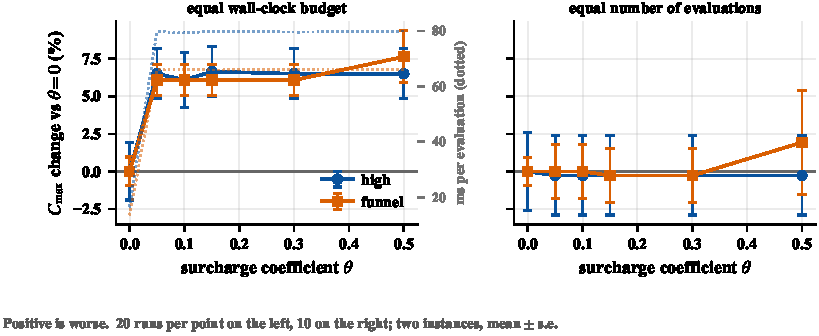
\includegraphics[width=\columnwidth]{fig/fig_theta.pdf}
\Description{Two panels of makespan change relative to theta equals zero against
surcharge coefficient: under equal wall-clock the penalty is large and flat, under
equal evaluations it is absent. Markers are means over seeds and error bars are
the standard error of the mean. The batch is two separately generated instances
that are not members of the paper's A/B/C families.}
\caption{Surcharge on corridor--time slots. A positive value means worse. Under equal wall-clock time (left), the makespan worsening appears as soon as the surcharge is turned on, then stays flat over a ten-fold range of $\theta$, in step with the cost per evaluation on the right axis; under an equal number of evaluations (right), the worsening disappears.
The damage comes from a higher cost per evaluation and hence fewer evaluations within the same budget, not from the surcharge choosing wrong paths.
Markers are means and error bars are the standard error of the mean; the number of runs per point is given in the figure footer. ``Significant'' refers to a two-sided Wilcoxon signed-rank test of each $\theta$ against $\theta=0$, paired by seed.
The two instances do not belong to the three families of Table~\ref{tab:instances}, and the legend labels \texttt{high}/\texttt{funnel} are layout tags only; see Table~\ref{tab:batches} for the batch.}
\label{fig:theta}
%% 由 fig/fig_theta_CN.py 从 clbs/experiments/theta_sweep.csv 与 theta_sweep_gen.csv 生成
%% (08-05 落盘,2 算例 x 10 种子,左图每点 20 次运行、右图 10 次)。
%% 更正:先前此处标注为"数据未落盘",实为误记——两个 CSV 均在盘上,已重新出图核对,
%% 图上形态与本小节正文一致(同挂钟下每个 theta 都变差且在十倍范围内平坦,同评价次数下归零)。
%% 该批次同属降本之前的测量,与第 5.5 小节引用的矩阵批次同期;定价机制在降本前后未改动,
%% 且其开销与剪枝无关(剪枝作用于派车试探,不作用于多标签路由),故该测量对它依然有效。
\end{figure}

The measurements are shown in Figure~\ref{fig:theta}. Under equal wall-clock time, every $\theta$ tried makes the makespan worse, and significantly so; the worsening is flat over a ten-fold range of $\theta$. Under an equal number of evaluations, the same comparison cannot be distinguished from zero.
Routing with a surcharge completes about one fifth as many evaluations within the same budget as routing without it: the surcharge does not mis-rank candidate solutions, but it sharply reduces the number of evaluations within the same budget.

Two further observations rule out other explanations. First, $\theta$ is not an effective tuning parameter on this problem. Over two orders of magnitude, routing with a surcharge modifies the same few paths, and both the cumulative surcharge and the returned makespan stay the same. The cumulative surcharge is only a small fraction of total travel time, not enough to change the order of arrival times in $\text{arrival time}+\theta\cdot\text{surcharge}$. Only when $\theta$ is so large that the surcharge outweighs the arrival time does the double counting take effect, and then makespan worsens sharply.
Second, the overhead is structural and is not caused by a non-zero surcharge. The runtime ratio of the same decode with and without a surcharge is the same at every $\theta$; the extra cost comes from ``maintaining a Pareto front at every node and trying several entry times on every arc'', regardless of whether a surcharge is actually applied. This agrees with Lemma~\ref{lem:label}: once a second criterion is introduced there is no longer a total-order dominance, and single-label search must be replaced by multi-label search.

The two budget conventions disagree on the size of the loss but agree on its sign. Whether the surcharge comes from a finite difference of corridor capacity or from a critical-chain proxy, the delay it targets is already counted in the arrival time of the yielding vehicle. As long as fitness is taken from a complete conflict-free decode, the surcharge carries no new information, and the comparison is decided by the overhead of the multi-label search it requires.
Hence, before extending the inter-layer interface, one should first check whether the objective of the receiving layer already contains the quantity the interface would pass; if it does, such an extension is harmful under our protocol.

%% 由独立小节降为上一节的子小节:它是消融的机制解释,不是本文的一级结论。
\subsubsection{Dilution and overhead}
\label{sec:whycost}

Why the yield record and staggering fail to offset their overhead can be established by measurement; the same measurement also explains why the overhead of reservation-table-aware dispatching had to be reduced first.

\paragraph{Allocation of decodes.}
Yield-record-guided local search consumes a large share of all decodes, yet fewer than one in fifty of the neighbours it decodes improve makespan. These improvements are real, but the same decodes spent on population evolution yield more.

The neighbourhood is small and well targeted by construction (Section~\ref{sec:ls}). A low improvement rate despite good targeting means that the operations named by the record do not shorten the critical chain after reassignment or staggering.
We tried three refinements: scoring reassignment by the expected yielding wait along the path rather than by unimpeded shortest-path time; replacing the adjacent swap of staggering with a directed insertion; and accepting plateau moves that ``leave makespan unchanged but lower total yielding wait''. Each was compared independently with the original operator under an equal number of evaluations, and \emph{none} was significant. The failure therefore lies in the signal itself, not in how the signal is used.

\paragraph{Dilution along the critical chain.}
A yield record names the corridor and the time slot of a yield and the transport that occupied that corridor first, that is, the information needed to remove \emph{that} event.
Makespan is determined by a chain. Once one corridor delay is removed, another constraint (an upstream operation, a robotic arm, or another corridor) usually becomes tight, so the realized improvement is only part of the delay removed.
This is why the acceptance rule re-extracts the critical chain after every acceptance. When a bottleneck is only one of several of comparable magnitude, feedback that names it improves makespan by far less than the yielding time it removes.

\paragraph{Why dispatching gives different results before and after the speed-ups.}
The same dilution acts on reservation-table-aware dispatching. The trial query selects the vehicle that delivers the current task earliest, which is a local improvement; only part of it survives when it propagates through the whole critical chain to makespan.
After dilution the reduction is still positive, but only a few percentage points. Before the speed-ups, a single evaluation cost \CostMultBefore{} times as much as under rule-based dispatching, too few evaluations fit into the same wall-clock time, and the net effect could not be distinguished from noise (the independent batch of Section~\ref{sec:whichcongestion}).
Only after Section~\ref{sec:speedup} lowered the cost to \CostMultAfter{} times did this reduction become significant in the pooled data.

Under a fixed budget, two quantities that can be measured and improved separately must be considered together: the makespan reduction that remains after dilution, and the extra cost per evaluation.
The two mechanisms fail for different reasons. Yield-record-guided local search is limited by the former: too little reduction survives dilution, and none of the three neighbourhood refinements reaches significance under an equal number of evaluations.
Dispatching is limited by the latter: the post-dilution reduction is always present, and it was initially not significant because the cost per evaluation was too high, a cost that can be lowered without changing the selected vehicle or the timetable.
This paper therefore lists dispatching as a mechanism contribution and reports yield-record-guided local search only as a controlled negative control.


\subsection{The cost law and the effect of the two speed-ups}
\label{sec:costlaw}

Under a fixed wall-clock budget, the cost per evaluation and the number of evaluations trade off against each other. The same dispatching rule has a net effect indistinguishable from noise before the speed-ups and significantly positive after them, so this section measures both quantities directly.

\paragraph{Two budget conventions.}
Figure~\ref{fig:protocol} shows the cost per evaluation of each configuration and the number of evaluations actually completed within the same budget cap. The cost spans about two orders of magnitude: cheaper configurations complete more evaluations, and the open loop completes the most evaluations while using only about one fifth of the wall-clock time.
Comparing at an equal number of generations lets the more expensive configuration use more compute; aligning wall-clock time lets the cheaper configuration complete more evaluations. We therefore report both conventions.

\begin{figure}[t]
\centering
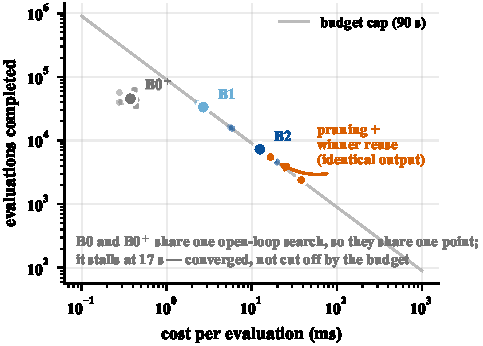
\includegraphics[width=\columnwidth]{fig/fig_protocol.pdf}
\Description{A log-log scatter of cost per evaluation against evaluations
completed. A grey hyperbola marks the 90-second budget cap. The two closed-loop
configurations sit on it, while the open-loop configuration sits well below it
because it stalls after about seventeen seconds. Orange markers are the
pruning ablation off and on; a callout marks the on setting.}
\caption{A fixed wall-clock budget places the cost per evaluation and the number of evaluations completed on a hyperbola; the grey line is the $90$-second cap shared by all configurations.
A point on the line means that cost $\times$ count equals that configuration's wall-clock time. The two closed-loop configurations lie on the line, that is, every run uses the full budget. The open loop lies \emph{below} it: it stops improving after a little over four hundred generations and is ended by early stopping, converging in about $17$ seconds rather than being cut off by the budget (Section~\ref{sec:protocol}).
B0 and B0$^+$ share the same open-loop search and therefore share one point; they differ only in how the schedule is executed. Pale small points are the individual measurements on three instances, and the large filled point is their geometric mean: on a log axis, only the geometric mean preserves ``cost $\times$ count $=$ that configuration's wall-clock time''.
Orange markers are the off and on settings of pruning and winner-path reuse (the callout marks the ``on'' setting). By Proposition~\ref{prop:speedup_equiv} the two produce identical output, so the displacement along the line reflects only the compute saved.}
\label{fig:protocol}
%% 由 fig/fig_protocol_CN.py 生成(输出名 fig_protocol_CN),数据源 clbs/output/ladder_cost.csv
%% 与 prune_ablation.csv;后者缺失时脚本自动省略橙色圆点而不报错。
\end{figure}

Figure~\ref{fig:protocols} runs the same set of comparisons once under each convention. The equal-generation convention ignores the extra cost per evaluation and therefore favours the configuration with the higher cost per evaluation: reservation-table-aware dispatching relative to rule-based dispatching is \GainProbeSameGen{} ($p\PProbeSameGen$). Under equal wall-clock time, before the speed-ups, the same comparison gives only \GainProbeSameClock{} ($p\PProbeSameClock$), close to zero.
The equal-generation convention asks whether the extra routing computation improves the ranking in each generation; the equal-wall-clock convention asks whether makespan falls within the same time. Both questions are meaningful, but neither can stand in for the other.

\begin{figure}[t]
\centering
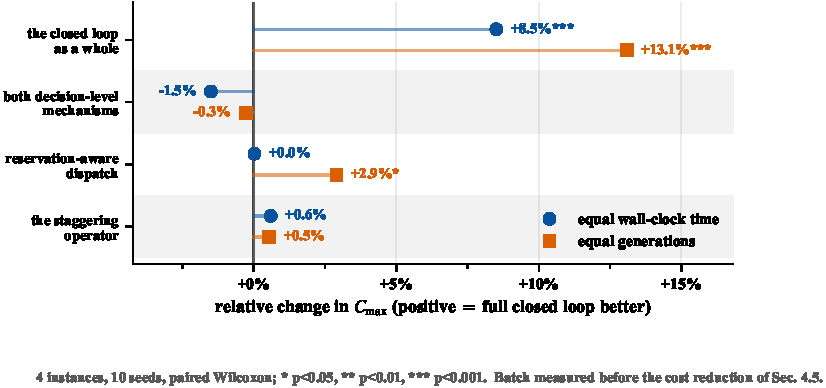
\includegraphics[width=\columnwidth]{fig/fig_protocols.pdf}
\Description{The same paired comparisons shown twice, once under an equal
wall-clock budget and once under an equal number of generations.}
\caption{The same set of comparisons under the two budget conventions. Each row is named by the mechanism it isolates.
The difference between the two markers comes from the convention: reservation-table-aware dispatching is \GainProbeSameGen{} ($p\PProbeSameGen$) at an equal number of generations and \GainProbeSameClock{} ($p\PProbeSameClock$), close to zero, at equal wall-clock time.
The batch ran before the two speed-ups (Table~\ref{tab:batches}), which is also why the speed-ups are switched on and off in a separate control below.}
\label{fig:protocols}
%% 由 fig/fig_protocols_CN.py 从 clbs/experiments/protocols.csv 生成(4 算例 x 10 种子)。
%% 行标签已从旧叙事的档位名(two-stage / open dispatch ...)改写为它所隔离的机制名,
%% 以免读者以为该图来自另一项研究;图脚已自报"降本之前"这一批次归属。
\end{figure}

\paragraph{The cost law.}
Reservation-table-aware dispatching raises the number of routing calls per transport task from $2$ to at most $2N_A$, so its cost grows linearly with fleet size.
The lower bound used by the pruning is tighter when contention is weaker, so more candidates are skipped; the larger the fleet and the stronger the contention, the smaller the cut.
The equivalence self-check of Section~\ref{sec:speedup} agrees with this direction: among its six instances, the highest cut rate in routing calls is on the least congested one (\RouteCallCutHi{}) and the lowest on the one with the largest fleet (\RouteCallCutLo{}); the pruning weakens but does not fail.
Together, the two trends \emph{predict} that when the fleet is large enough and contention strong enough, the growing trial-query cost will offset the gain. In Section~\ref{sec:whichcongestion}, the sign alternates across the four levels of the vehicle-to-arm ratio and none of the four instances is significant, so this upper bound is not confirmed.
The cost law itself (cost growing linearly with $N_A$, pruning effect falling with $N_A$) is measured directly; the upper bound derived from it has not yet been verified.

\paragraph{Switching the two speed-ups on and off.}
The speed-ups and the dispatching rule were introduced one after the other, so setting the two batches side by side cannot rule out the effect of differences in instances and baselines. We therefore run a separate control that changes only the speed-ups: same instances, same seeds, same budget, with pruning and winner-path reuse switched on or off.

Proposition~\ref{prop:speedup_equiv} guarantees that the two speed-ups \emph{do not change the selected vehicle or the timetable}. On each of six instances we take six random chromosomes; with the speed-ups on and off, the makespans and dispatch sequences are \emph{identical bit for bit} in all $36$ cases, without exception, and routing calls fall by \RouteCallCut{} in total. Since the output is identical, turning the speed-ups off only makes each evaluation slower, and any makespan difference under equal wall-clock time comes \emph{only} from the compute saved.

Table~\ref{tab:prune}: going from off$\to$on lowers makespan by a further \GainPrune{} (\WinPrune{} wins / \LosePrune{} losses, $p\PPrune$); the number of evaluations within the same budget is \EvalRatioPrune{} times as large, and a single evaluation runs \SpeedupProbe{} times faster.
This control links the two batches: the same rule gives \GainProbePre{} on the matrix batch before the speed-ups ($0$ of the $\MatrixCells$ instances significant) and is significantly positive on the ladder batch after them, while the speed-ups themselves change no selection.

\begin{table}[t]
\caption{Changing only pruning and winner-path reuse. ``Off''/``on'' indicates whether the two are enabled; the bold header marks the setting adopted in this paper.
The two settings produce bit-identical output (verified by the equivalence self-check), so the difference comes only from the compute saved. Same instances, same seeds, same wall-clock time; $n=60$ pairs, two-sided Wilcoxon signed-rank test ($^{***}p<0.001$); the aggregate row lists wins/losses/ties and $p$.
Both ratio columns use the \emph{off} value as denominator, in opposite directions: evaluations as on/off, time per evaluation as off/on.}
\label{tab:prune}
\small
%% 数字与 clbs/output/prune_ablation.csv / 运行日志一致;亦可用
%% py paper01/tab/gen_tables_ladder.py 从同一 CSV 重生成。
%% 由 tab/gen_tables_ladder.py 生成,请勿手工编辑
%% 数据源:clbs/output/baseline_ladder.csv 等,见脚本首部
\begin{tabular}{@{}lrrrrrr@{}}
\toprule
& & \multicolumn{2}{c}{$C_{\max}$ (time units)} & & Eval.\ count ratio & Speedup per eval. \\
\cmidrule(lr){3-4}
Instance & Contention & Off & \textbf{On} & $\Delta C_{\max}$ & (on/off) & (off/on) \\
\midrule
A funnel & 31.9\% & 44.80 & 42.10 & $-6.03\%$ & 2.21$\times$ & 2.23$\times$ \\
A high & 30.9\% & 41.60 & 37.70 & $-9.37\%$ & 2.40$\times$ & 2.41$\times$ \\
A low & 11.8\% & 60.50 & 57.00 & $-5.79\%$ & 2.79$\times$ & 2.81$\times$ \\
B NA/NM 0.5 & 15.8\% & 66.70 & 65.10 & $-2.40\%$ & 2.11$\times$ & 2.11$\times$ \\
B NA/NM 1.0 & 30.2\% & 51.90 & 48.90 & $-5.78\%$ & 2.31$\times$ & 2.31$\times$ \\
B NA/NM 2.0 & 32.4\% & 44.50 & 42.20 & $-5.17\%$ & 1.98$\times$ & 2.01$\times$ \\
\midrule
\emph{Pooled} (60 pairs) & --- & --- & --- & $-5.60\%^{***}$ & \multicolumn{2}{r}{50/0/10,\ $<10^{-4}$} \\
\midrule
\multicolumn{7}{@{}l@{}}{\footnotesize HL pseudomedian and $95\%$ CI:$-4.72$ $[-6.34,-3.55]$\,\%} \\
\bottomrule
\end{tabular}

\end{table}
\subsection{Case study: Gantt chart and critical chain on the funnel instance}
\label{sec:casestudy}

Aggregate numbers do not show what happens inside one solve. This section places B0 and B2 side by side on a single funnel instance and colours the links of the critical chain according to Table~\ref{tab:attrib}.

Figure~\ref{fig:case_gantt} draws the robotic arms and vehicles on a shared time axis; vehicle rows distinguish empty and loaded legs, and yielding waits are coloured separately. Three observations follow. In the open-loop solution, yielding waits appear in stretches on the corridors near the load/unload point and concentrate on a few vehicles. The closed-loop solution greatly reduces these waits, and several operations are assigned to an arm that is not the fastest, i.e.\ assignments of the kind described by Eq.~\eqref{eq:reassign}, which trade a longer processing time for a shorter path with better traffic conditions. The closed-loop solution also balances vehicle load more evenly; this is a consequence of the first two points rather than a separate mechanism.

\begin{figure*}[t]
\centering
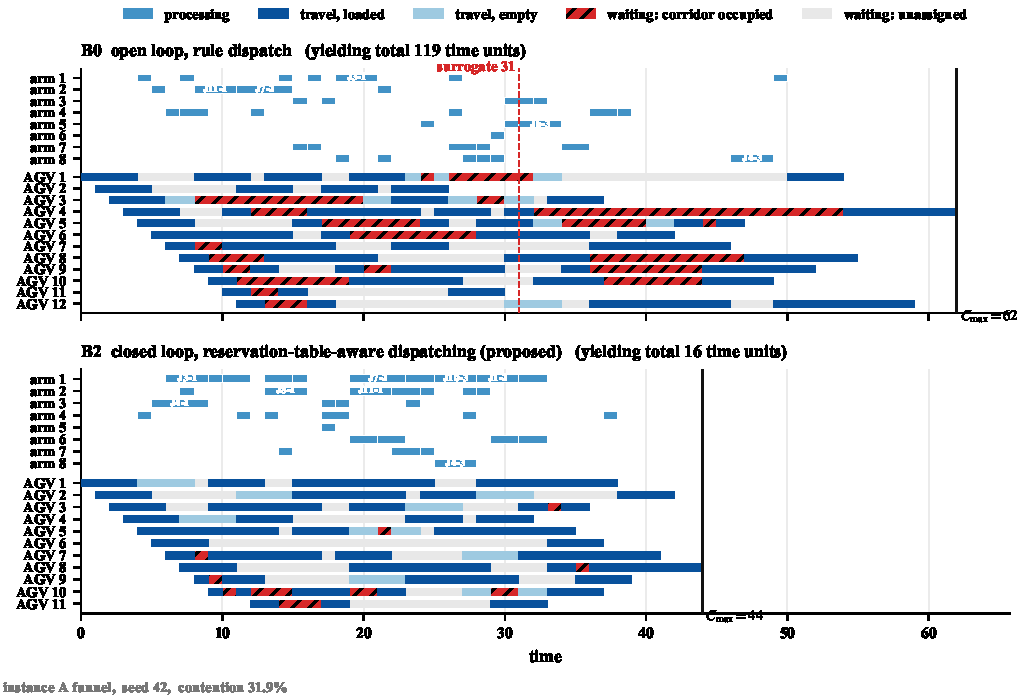
\includegraphics[width=\textwidth]{fig/fig_case_gantt.pdf}
\Description{Side-by-side Gantt charts of the open-loop and closed-loop
solutions on one funnel instance, with arms and vehicles on a shared time axis
and yielding waits shaded separately.}
\caption{B0 (top) and B2 (bottom) on the same funnel instance. Robotic arms and vehicles share the time axis; vehicle rows distinguish empty and loaded legs, as well as two kinds of gap.
A gap between the two legs of the same transport task: the vehicle waits at a berth because a corridor is occupied, i.e.\ a yielding wait, which is the delay treated in this paper.
A gap between different tasks: the vehicle is idle. The two are shown in different colours so that idle time is not misread as yielding.}
\label{fig:case_gantt}
%% 由 fig/fig_case_gantt_CN.py 从 clbs/output/case_study/*.json 生成(tools/ladder_diag.py
%% 的 --case-study 落盘)。让行/空闲的区分由脚本从相邻段的 task 字段推出,不是另存的标注。
\end{figure*}

Figure~\ref{fig:case_chain} colours each link by the five labels of Table~\ref{tab:attrib}. On the B0 chain, \texttt{corridor} links take a substantial share; on B2 they largely disappear and are replaced by \texttt{machine} and \texttt{upstream}.
This is the dilution described in Section~\ref{sec:whycost}: once a corridor delay is removed, another constraint becomes tight.

\begin{figure}[t]
\centering
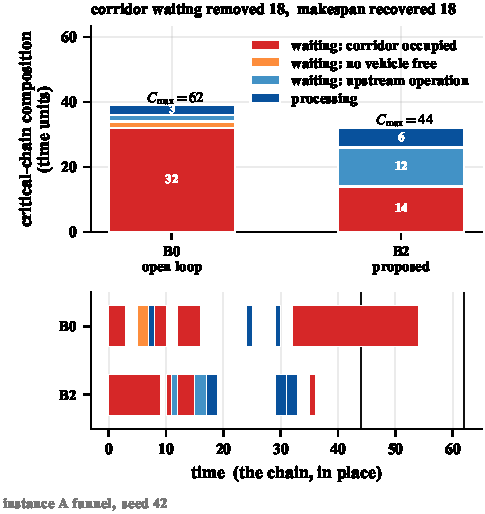
\includegraphics[width=\columnwidth]{fig/fig_case_chain.pdf}
\Description{The critical chain of the open-loop and closed-loop solutions,
with each link coloured by its attribution label.}
\caption{Links of the critical chain coloured according to Table~\ref{tab:attrib}. Top: composition of the B0 and B2 critical chains; the title places ``corridor wait removed'' beside ``makespan actually reduced'', and their difference is the part absorbed by the newly tight constraints.
Bottom: the same chain positioned on the time axis, showing that the bars above decompose one chain rather than forming a histogram of unrelated events.
In the closed-loop solution, \texttt{corridor} largely disappears and is replaced by robotic arms and upstream operations.}
\label{fig:case_chain}
%% 由 fig/fig_case_chain_CN.py 从同一批 case_study/*.json 生成;归因标签直接取
%% algorithm/decoder.py 的 critical_chain(),五类标签一个不并、不归入 other。
\end{figure}

\subsection{Degenerate comparison on public benchmarks}
\label{sec:external}

All preceding sections compare different configurations of the same implementation on self-generated instances. This excludes implementation differences among configurations but cannot calibrate the absolute level of the implementation: even if the upper-level search is weak, the differences among configurations remain credible, whereas the absolute makespan reflects only the level of the implementation. This section calibrates the upper-level search on public benchmarks.

\paragraph{What is compared.}
Once the exclusivity constraint, Eq.~\eqref{eq:excl}, is removed, our model degenerates exactly to the standard FJSP\_PT (Section~\ref{sec:Chapter_III}), which is the \emph{same mathematical problem} as the public benchmarks. We additionally set $\delta_{\mathrm{ret}}=0$ to match the makespan definition of these instances; this is a model parameter (Table~\ref{tab:notation}), not the removal of a further constraint.
After degeneration there is no corridor contention and neither mechanism comes into play, so what is tested is the \emph{upper-level search}, not our framework. The results are reported in a table separate from the self-generated instances, so that the two conclusions do not share one table.

\paragraph{Instances and protocol.}
We take the \PubNInst{} instances compiled by Homayouni and Fontes~\cite{homayouni2021production} (originating from Fattahi et al.~\cite{fattahi2007mathematical}; $2$--$12$ jobs, $4$--$48$ operations, $2$--$8$ machines) and, following the setting of Lim and Moon~\cite{lim2023twophase}, use two vehicles with no return of finished products. Travel times are taken \emph{as published} from the released matrices, without shortest-path synthesis: Section~\ref{sec:instances} has noted that \PubNLayoutBad{} of these matrices are not the shortest-path closure of any graph, so synthesis would alter the instances.
After degeneration the road network $G$ enters the model only through $t^{*}$, so the published matrix can be used directly as $t^{*}$ without requiring a consistent $G$ to exist. Contention requires $G$ itself, which these instances do not provide, so they can be used \emph{only} in the degenerate setting.
For two small instances (\textsc{sfjst}01, \textsc{sfjst}03), the published optima were verified digit by digit by hand, confirming that neither includes a return trip.
Reference values: \PubNOpt{} instances have a MILP-proven optimum~\cite{homayouni2021production}, and for the remaining $4$ we use the best published values~\cite{lim2023twophase}.

\paragraph{Results.}
Table~\ref{tab:external} covers \PubNInst{} instances $\times$ \NSeeds{} seeds. All $200$ runs pass three checks: no solution falls below the composite lower bound, no validation fails, and on the \PubNOpt{} instances with a proven optimum ($160$ runs) no run falls below that value. Because the degenerate setting and the literature pose the same problem, this verifies that the conversion and the conventions are correct.
On $\PubNMatch{}/\PubNInst{}$ instances the best solution is \emph{identical digit for digit} to the reference value, including all $10$ small instances (\textsc{sfjst}01--10); the mean gap over the \PubNInst{} instances is \PubGapMean{} (median \PubGapMed{}).
The gap rises with size, but not monotonically from one instance to the next: \textsc{mfjst}03 and \textsc{mfjst}06 both do better than their respective smaller neighbours. The four largest instances ($32$--$48$ operations) average \PubGapBig{}, with a worst case of \PubGapMax{}; none of the $16$ instances with at most $24$ operations exceeds $5.45\%$.

\begin{table}[t]
\caption{Degenerate comparison on public benchmarks (exclusivity constraint removed; the same problem as in the literature). In the ``reference'' column,
\textsc{opt} denotes a MILP-proven optimum and \textsc{bk} a best published value; the gap is computed from the best
solution over \NSeeds{} seeds. An asterisk marks instances whose best solution is identical digit for digit to the reference value.}
\label{tab:external}
\centering
\small
%% 由 tab/gen_tables_ladder.py 生成,请勿手工编辑
%% 数据源:clbs/experiments_database/gap_ideal.csv;工序数取自 clbs/database/json/hf/*.json
\begin{tabular}{lrrrrrr}
\toprule
& & & \multicolumn{3}{c}{$C_{\max}$ (time units)} & \\
\cmidrule(lr){4-6}
Instance & Ops & Ref. & \multicolumn{1}{c}{Value} & Best & Mean & Gap \\
\midrule
SFJST01 & 4 & \textsc{opt} & 70 & 70\rlap{$^*$} & 70.0 & 0.00\% \\
SFJST02 & 4 & \textsc{opt} & 111 & 111\rlap{$^*$} & 111.0 & 0.00\% \\
SFJST03 & 6 & \textsc{opt} & 223 & 223\rlap{$^*$} & 223.0 & 0.00\% \\
SFJST04 & 6 & \textsc{opt} & 359 & 359\rlap{$^*$} & 359.0 & 0.00\% \\
SFJST05 & 6 & \textsc{opt} & 123 & 123\rlap{$^*$} & 123.0 & 0.00\% \\
SFJST06 & 9 & \textsc{opt} & 324 & 324\rlap{$^*$} & 324.0 & 0.00\% \\
SFJST07 & 9 & \textsc{opt} & 409 & 409\rlap{$^*$} & 409.0 & 0.00\% \\
SFJST08 & 9 & \textsc{opt} & 269 & 269\rlap{$^*$} & 269.5 & 0.00\% \\
SFJST09 & 9 & \textsc{opt} & 220 & 220\rlap{$^*$} & 222.0 & 0.00\% \\
SFJST10 & 12 & \textsc{opt} & 531 & 531\rlap{$^*$} & 531.0 & 0.00\% \\
MFJST01 & 15 & \textsc{opt} & 485 & 485\rlap{$^*$} & 485.0 & 0.00\% \\
MFJST02 & 15 & \textsc{opt} & 463 & 476 & 483.4 & 2.81\% \\
MFJST03 & 18 & \textsc{opt} & 482 & 482\rlap{$^*$} & 504.7 & 0.00\% \\
MFJST04 & 21 & \textsc{opt} & 576 & 586 & 623.0 & 1.74\% \\
MFJST05 & 21 & \textsc{opt} & 532 & 561 & 592.8 & 5.45\% \\
MFJST06 & 24 & \textsc{opt} & 652 & 677 & 728.3 & 3.83\% \\
MFJST07 & 32 & \textsc{bk} & 898 & 965 & 1023.3 & 7.46\% \\
MFJST08 & 36 & \textsc{bk} & 900 & 970 & 1027.0 & 7.78\% \\
MFJST09 & 44 & \textsc{bk} & 1098 & 1226 & 1279.2 & 11.66\% \\
MFJST10 & 48 & \textsc{bk} & 1230 & 1389 & 1473.0 & 12.93\% \\
\bottomrule
\end{tabular}

\end{table}
%% 由 tab/gen_tables_ladder.py 的 tab_external() 从
%% clbs/experiments_database/gap_ideal.csv 生成;"工序"列是全表唯一不在该 CSV 里的
%% 量,由脚本从 clbs/database/json/hf/*.json 现数(len(proc_time)),不得手填。
%% 同一函数还打印 \PubNInst、\PubNOpt、\PubNMatch、\PubGapMean、\PubGapMed、
%% \PubGapMax、\PubGapBig、\PubGapMeanSeed、\PubLBSlack、\PubLBTotal 十个导言区宏,
%% 故本小节的表与正文同源。改表前先改 CSV,再重跑脚本。

\paragraph{The gap stems mainly from search capability, not from an insufficient budget.}
Among the \PubNOpt{} proven optima in the literature, the MILP on the largest instance took nearly ten hours (\textsc{mfjst}06, $34\,796$ seconds), whereas each of our runs takes only a few seconds. We therefore raised the budget (generation cap five times, early-stopping threshold $3.3$ times, measured wall-clock time increased to \PubBudgetRatio{} times) and re-ran the $10$ \textsc{mfjst} instances in the last ten rows of Table~\ref{tab:external}---which is where the gaps concentrate.
The mean gap of these ten instances falls from \PubGapLoBudget{} to \PubGapHiBudget{} (the base contains only these ten, a different basis from the \PubGapMean{} over the \PubNInst{} instances above); that is, \PubBudgetRatio{} times the computation yields an improvement of only $\PubBudgetGainPP$ percentage points. \PubBudgetNoGain{} of them show no decrease, and the instance with the largest gap falls from $12.93\%$ to $12.85\%$.
Under both budgets, \emph{none} of the $300$ runs reaches the generation cap; all are terminated by early stopping, so the larger budget did not lengthen the search. The gap therefore mainly reflects the capability limit of the upper-level search. Narrowing it on large instances is item~(3) of Section~\ref{sec:future_work}.

\paragraph{Sources of the gap between the composite lower bound and the best solution.}
The median gap between the composite lower bound and the best solution found is \LBGapMed{}. This gap has two components: the amount by which the bound lies below the true optimum, and the amount by which the search solution lies above it. On the self-generated instances the optimum is unknown, so the two components cannot be separated.
On the public instances they can. We take only the \PubNOpt{} instances with a proven optimum: the reference of the other $4$ is a best published value, the true optimum can only be smaller, and using it as the denominator would overestimate ``how far the bound lies below the optimum''.
On these \PubNOpt{} instances, the same composite lower bound lies a median \PubLBSlack{} below the proven optimum and a median \PubLBTotal{} below our best solution; taking the difference instance by instance, the search solution lies a median $\PubLBResidMed$ percentage points above the optimum (most instances hit the optimum), and at most $\PubLBResidMax$ percentage points.
Hence, on these \emph{contention-free} instances, almost all of the gap between the bound and the best solution comes from slack in the bound, not from the search failing to find the optimum.
This proportion cannot be transferred directly to the self-generated instances. The composite lower bound is constructed without corridor contention; on the self-generated instances the true optimum can only rise or stay the same because of contention while the bound does not change, so the distance between the bound and the true optimum is no smaller than on the public instances.
What can be established is that the \LBGapMed{} on the self-generated instances \emph{cannot} be read as a search gap, because the same bound already lies \PubLBSlack{} below the optimum without contention. The distance between the search and the optimum on the self-generated instances remains unknown (Limitation~(3) in Section~\ref{sec:limitations}).



\section{Conclusion}

This paper studies scheduling problems in which flexible assignment and conflict-free AGV routing must be decided together, focusing on shops where transport takes longer than processing and congestion concentrates on a few shared corridors: in such shops, when the corridor to a fast arm is congested, a slower robotic arm with better traffic conditions may be the better assignment. Our bilevel framework lets information from lower-level routing enter decisions through two paths, evaluation and dispatching, and measures the gain and cost of each separately under the same wall-clock budget. The main conclusions are as follows.


\subsection{Summary}
\label{sec:contributions}

\textbf{(1) Instance families with controllable contention intensity.}
Three families of controlled instances, varying layout, vehicle-to-arm ratio, and flexibility, allow contention intensity to be varied on its own. On them, the closed-loop gain broadly rises with contention intensity, and on the most congested instance it is about two and a half times that on the least congested one, but the relationship is not monotonic (Section~\ref{sec:whichcongestion}).

\textbf{(2) A closed-loop bilevel framework with routing-in-the-loop evaluation.}
The upper level searches assignment and sequencing with a memetic algorithm, and the lower level performs conflict-free routing by time-window reservation; the fitness of each candidate solution is the makespan after the lower level has completed all transports.
Proposition~\ref{prop:decodable} and Lemma~\ref{lem:label} guarantee that every chromosome is decodable and that the evaluation is consistent with the conflict model of Section~\ref{sec:Chapter_III}, with no repair operator needed.
Relative to the open loop, the closed loop reduces makespan by $\GainLoopRule$ ($p\PLoopRule$) under rule-based dispatching and by $\GainLoopProbe$ ($p\PLoopProbe$) under reservation-table-aware dispatching.

\textbf{(3) Reservation-table-aware dispatching and two speed-ups that do not change the output.}
Before a vehicle is selected, a trial query on the reservation table is run for both transport legs, and the earliest feasible delivery time replaces the unimpeded shortest-path estimate; within the closed loop this reduces makespan by a further $\GainProbeLoop$ ($p\PProbeLoop$).
The rule raises the cost per evaluation to \CostMultBefore{} times that of rule-based dispatching, enough to offset its gain under the same wall-clock budget. Admissible lower-bound pruning and winner-path reuse change neither the selected vehicle nor the timetable (Proposition~\ref{prop:speedup_equiv}, also confirmed by a bitwise self-check on six instances); they cut router calls by \RouteCallCut{} and lower the cost multiple to \CostMultAfter{}.

\textbf{(4) The two paths differ in magnitude, each is effective, and neither can substitute for the other.}
The closed loop remains significant after Holm correction on \CellsSigLoopAdj{} of the $\NCases$ instances; reservation-table-aware dispatching is significant under both the open and the closed loop only when the instances are pooled for testing ($\GainProbeOpen$, $p\PProbeOpen$; $\GainProbeLoop$, $p\PProbeLoop$, $95\%$ interval \CIProbeLoop{}).
The end-to-end gain $\GainEndToEnd$ is slightly below the prediction under independent composition, $\GainIndepProduct$; the two mechanisms do not amplify each other.
The ``schedule first, then resolve conflicts'' route can obtain only the open-loop dispatching gain of $\GainProbeOpen$; because its first-stage search does not count yielding, the reduction corresponding to closed-loop evaluation ($\GainLoopRule$) is unavailable to it.


\subsection{Limitations}
\label{sec:limitations}

\textbf{(1) Scope of the instance families, and why self-generated instances are used.}
The main experiment fixes the size and varies only the structure (Section~\ref{sec:features}), so we draw no conclusion about how the mechanisms vary with size. Heterogeneity $H$ is fixed at $0.3$; the scan over four $H$ levels comes from the smaller, independent instances of Section~\ref{sec:whichcongestion}, so ``the gain does not rise with $H$'' holds only at \emph{that} size.
The layout family combines two topologies: the three spine instances vary only network capacity, whereas the two grid instances vary topology and distance together (the farthest leg rises from \LegDumbbell{} to \LegGrid{}, Section~\ref{sec:instances}). Moreover, the contention intensity used to characterize this family is a one-dimensional measure that does not separate the part of yielding that reassignment can bypass.
Hence only the differences among the three spine instances can be attributed to capacity alone, and the five instances should not be joined into one curve by contention intensity; these two points are also possible reasons why the gain and contention intensity are not in strictly the same order.
Self-generated instances are used because this direction has no public benchmark with an explicit road network (Section~\ref{sec:instances}).

\textbf{(2) The makespan gain from dispatching is positive on average, but the class of instances on which it appears stably cannot yet be determined.}
$\NSeeds$ seeds per instance suffice to resolve the closed-loop effect (significant on $\CellsSigLoopAdj$ of the $\NCases$ instances after Holm correction). The effect of reservation-table-aware dispatching is only a few percentage points, of the same order as the dispersion across seeds: of the $\NCases$ instances, $\CellsSigProbe$ are significant before correction and $\CellsSigProbeAdj$ after.
The gain can therefore be confirmed as positive only on the $\NPairs$ pooled pairs ($95\%$ interval \CIProbeLoop{}, whose lower end is less than one percentage point from zero).
Raising the number of seeds by about an order of magnitude would be needed to determine the class of instances on which it appears and to test the fleet-size upper bound predicted by the cost law of Section~\ref{sec:costlaw}.

\textbf{(3) The upper-level search has been calibrated on contention-free public benchmarks; with corridor contention, the distance of solutions from the optimum cannot yet be determined.}
All configurations share one implementation, and what is reported are the differences among configurations; the strength of the upper-level search is common to all configurations and does not affect those differences. The degenerate comparison of Section~\ref{sec:external} matches the literature digit for digit on $\PubNMatch{}/\PubNInst{}$ instances, and all $10$ small instances reach the proven optimum. The gap rises with size: the four largest instances average \PubGapBig{}, and \PubBudgetRatio{} times the computation improves it by only $\PubBudgetGainPP$ percentage points, so the gap reflects a capability limit rather than an insufficient budget.
On the \PubNOpt{} public instances with a proven optimum, the search solution is at most $\PubLBResidMax$ percentage points from the optimum, and the bound gap comes almost entirely from slack in the bound. On the self-generated instances the composite lower bound contains no contention, so its median gap \LBGapMed{} to the best solution cannot be read as a search gap; we draw no quantitative conclusion about this distance.
The public instances contain no corridor contention, and lower-level routing with the reservation table has no proven optimum to compare against; the much smaller effect of a few percentage points (such as \GainProbeLoop{}) may be of the same order as the distance of the implementation from the optimum.

\textbf{(4) The surcharge and yield-record-guided local search did not further reduce makespan; if their evaluation cost is reduced on its own, they must be remeasured.}
Both were assessed in the same implementation under the same wall-clock budget, so what was measured is the trade-off between cost per evaluation and number of evaluations: when all configurations are sped up by the same factor, that trade-off and the sign of the conclusion stay unchanged; only reducing the cost of one interface on its own could change the sign, as the dispatching speed-ups of Section~\ref{sec:speedup} illustrate.
Hence, if neighbourhood evaluation is changed to re-solve only the perturbed part, they must be remeasured (item~(4) of Section~\ref{sec:future_work}).

\textbf{(5) Dynamic disruptions such as robotic-arm and vehicle failures are not considered.}
Assumption A7 already excludes robotic-arm and vehicle failures and dynamic job arrivals from the model. The reported results are limited to the static setting in which the job set and processing times are known over the planning horizon and equipment does not fail. Under failures or online arrivals, the value of a mechanism also includes how fast it repairs a schedule, not only the quality of the schedule it constructs; this aspect is not measured here (item~(5) of Section~\ref{sec:future_work}).

\subsection{Future work}
\label{sec:future_work}

\textbf{(1) Remeasure on larger explicit road networks, and separate contention from chain substitutability.}
This corresponds to Limitation~(1). Since the main experiment fixes the size, the first step is to test on larger explicit corridor networks whether the closed-loop and dispatching gains keep the same magnitude. In layout design, ``whether congestion can be bypassed by reassignment'' and ``whether the critical chain has only one dominant bottleneck'' should be treated as two independent factors; the current contention intensity is a one-dimensional measure that does not separate congestion bypassable by reassignment, so a new measure, first validated on instances whose answers are known, is needed.

\textbf{(2) Raise the number of seeds to determine the class of instances on which the dispatching gain appears stably.}
This corresponds to Limitation~(2). The makespan gain from dispatching has been confirmed to be positive on average. Raising the number of seeds by about an order of magnitude and sampling the vehicle-to-arm ratio at denser levels would determine the class of instances on which it appears stably and test the cost law: whether there is a fleet size beyond which the growth in trial-query cost offsets the gain.

\textbf{(3) Measure the distance of solutions from the optimum on instances with corridor contention.}
This corresponds to Limitation~(3). The \PubGapBig{} on the large public instances is insensitive to longer search time, the standard deviation across seeds on the four instances reaches \PubCvBig{} of the mean, and all runs are terminated by early stopping, so it is the encoding or the neighbourhood that needs improvement.
At the small end, exact solutions obtained with the logic-based Benders decomposition of van Os and Basten~\cite{vanos2026exact} would separate, under corridor contention, the shares due to bound slack and to insufficient search, and would test whether the surcharge and yield-record-guided local search still fail to reduce makespan under a stronger search.
A stronger search does not affect the differences among configurations, but may help determine the class of instances on which the dispatching gain appears stably (Limitation~(2)).

\textbf{(4) Reduce cost by incremental evaluation, then remeasure yield-record-guided local search.}
This corresponds to Limitation~(4). The decoder state advances in one direction, so when a perturbation acts only on the sequence after some position, earlier events and reservations are unchanged. Re-solving only the perturbed part amounts to reducing the cost per evaluation of this kind of local search on its own, after which it can be remeasured under the same wall-clock budget.

\textbf{(5) Measure the speed of schedule repair under robotic-arm and vehicle failures.}
This corresponds to Limitation~(5). Work on the dynamic flexible job shop has already brought machine failures, rush orders, and job arrivals into rescheduling~\cite{gui2023dynamic,xiong2024dynamic,dauzereperes2024fjsp}.
In that case the value of a mechanism also includes the speed of repairing a schedule, not only the time and quality of constructing one. Whether an evaluator that re-solves from scratch or a method that modifies only a local neighbourhood holds the advantage cannot be carried over directly from conclusions in the static setting.


%\section*{Acknowledgments}
%This work was supported partly by Key Laboratory of Computer Network and Information Integration (Southeast University) of Ministry of Education of China under Grants NO. 93K-9 and Jiangsu Provincial Key Laboratory of Network and Information Security under Grants No.BM2003201.

%%
%% The next two lines define the bibliography style to be used, and
%% the bibliography file.
\bibliographystyle{ACM-Reference-Format}
\bibliography{reference-base}


%% 本文没有附录。acmart 的 \appendix 若不带任何内容会在目录与页眉里留下一个空标题,
%% 故直接不声明;若日后要加附录,在此处恢复 \appendix 再写 \section。

\end{document}
\endinput
%%
